En este capítulo se analizará el uso de la plantilla de \acrfull{tfg}. Además de los elementos propios de la plantilla se presentarán los elementos básicos de \gls{latex}.

\section{Plantilla}\label{sec:plantilla}


La plantilla consta de varios ficheros. El fichero principal es \texttt{main.tex}. Además, hay otros ficheros en la carpeta \texttt{config}. En principio no es necesario tocar estos ficheros.


En el fichero principal hay varias cosas que se pueden configurar.

Lo primero, la plantilla se basa en el estilo \texttt{memoir}. Por tanto, es posible usar todas las opciones asociadas a dicho estilo. Principalmente, se puede cambiar el estilo de los capítulos. Para ello, en el fichero \texttt{main.tex} al comienzo hay un comando, \texttt{chapterstyle}, con el que se puede definir el estilo. Estas son las opciones disponibles.
\begin{itemize}
	\item bianchi
	\item bringhurst
	\item brotherton
	\item chappell
	\item crosshead
	\item culver
	\item dash
	\item demo2
	\item demo3
	\item dowding
	\item ell
	\item ger
	\item komalike
	\item lyhne
	\item madsen
	\item ntglike
	\item pedersen
	\item southall
	\item tandh
	\item thatcher
	\item veelo
	\item verville
	\item wilsondob
\end{itemize}

\subsection{Información sobre el proyecto}

En el fichero \texttt{information.tex} encontramos los comandos para definir la información general del trabajo: autor/a, título, director/a/es/as, fecha del documento, titulación, etc.

\subsection{Idioma del documento}

El documento puede estar en castellano, euskara o inglés. Para configurar adecuadamente todos los cambios necesarios, en el fichero \texttt{information.tex} se puede definir el idioma descomentando la opción adecuada y comentando el resto. Solo una de las opciones debe estar descomentada.

\begin{table}[h]
	\centering
	\begin{tabular}{l|llll}
		Y & A & B & C & D\\
		\hline
		y1 & a1 & b1 & c1 & d1\\
		y2 & a2 & b2 & c2 & d2\\
	\end{tabular}
	\caption {Ejemplo de tabla}\label{tab:ejemplo}
\end{table}


% Más info: https://www.tablesgenerator.com/

\subsection{Contenido del documento}

A fin de facilitar la organización del texto el contenido está dividido en ficheros por capítulos en la carpeta \texttt{chapters}. A pesar del que el código está en dichos ficheros, a fin de tener una idea clara de la organización el título de los capítulos se define en el fichero \texttt{main.tex}.

\section{Figuras y tablas}

\begin{figure}[t]
    \centering
	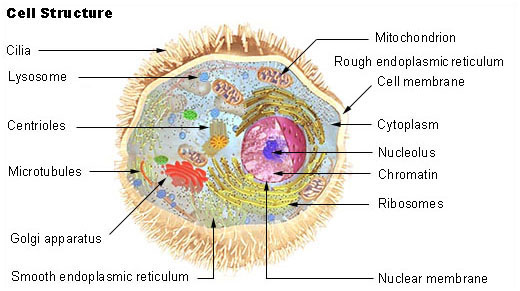
\includegraphics[width=0.75\textwidth]{figures/cell.jpg}
	\caption{Ejemplo de una imagen}\label{fig:ejemplo}
\end{figure}

Con el objetivo de mantener el aspecto del documento se recomienda que las figuras y tablas estén todas arriba o abajo. Para ello es necesario usar las opciones \texttt{[t]} o \texttt{[b]} en los entornos \texttt{figure} y \texttt{table}.

La Figura \ref{fig:ejemplo} y la Tabla \ref{tab:ejemplo} muestran dos ejemplos. Hay que tener en cuenta que \LaTeX trata de optimizar la localización de la figuras y tablas. Como se ha mencionado, es recomendable seguir un criterio fijo (todas arriba o todas abajo). Para cambiar la hoja en la que aparece una figura o tabla hay que mover de lugar su código. Dicho código no tiene por que estar donde se menciona en el texto, ya que la referencia a las figuras y tablas debe hacerse usando su número y no usando términos como ``abajo'' o ``arriba''.

\section{Algoritmos y fragmentos de código}

El algoritmo \ref{alg:ejemplo} muestra un ejemplo de algoritmo.

\clearpage

\begin{algorithm}
\caption{Ejemplo de un algoritmo}\label{alg:ejemplo}
\begin{algorithmic}
\Require $n \geq 0$
\Ensure $y = x^n$
\State $y \gets 1$
\State $X \gets x$
\State $N \gets n$
\While{$N \neq 0$}
\If{$N$ is even}
    \State $X \gets X \times X$
    \State $N \gets \frac{N}{2}$
\ElsIf{$N$ is odd}
    \State $y \gets y \times X$
    \State $N \gets N - 1$
\EndIf
\EndWhile
\end{algorithmic}
\end{algorithm}

Existen varios paquetes para introducir fragmentos de código. Esta plantilla utiliza el paquete \texttt{lstlisting}.\footnote{Más información en \cite{lstlistingdoc}.} Por norma general, no se suele incluir código en el cuerpo de la memoria, a menos que sea transcendental para la comprensión del trabajo. A continuación se muestran algunos ejemplos de fragmentos de código. El estilo (colores, borde, etc.) está definido en el fichero \texttt{config/macros.tex}.

Fragmento de código de Java.
\begin{lstlisting}[language=Java]
public static void main(String args[]) {
    for(int i = 0; i <= 12; i++) { // comentario
        System.out.print("12 * "+ i + " = " + 12 * i + "\n");
    }
}
\end{lstlisting}

Fragmento de código de SQL, sin números de línea.
\begin{lstlisting}[language=SQL,numbers=none]
select *
from proyectos
where calificacion between 8 and 10
\end{lstlisting}


\section{Referencias}

Para añadir la bibliografía hay que usar BibTeX. Las referencias están recogidas en el fichero \texttt{references.bib} y en el texto se citan usando el comando \texttt{cite}. Por ejemplo, \cite{Shahbaba2011} o \cite{Efron1994, Rmanual, Subramanian2005gene}. No hay que olvidar añadir toda la información de las referencias (páginas, año, etc.). 